\section{Execution Model}
\label{sec:execution}

The stack utilizes a multi-tasking execution model managed by the \textbf{VAIOS} (Vayu Input/Output System) real-time kernel. This model ensures that high-frequency control loops, asynchronous communication, and background maintenance tasks coexist on a single microcontroller while satisfying strict real-time constraints.

\subsection{Task Scheduling and Priorities}

The system organizes functionality into discrete tasks, each assigned a priority level and an execution frequency. VAIOS employs a priority-based preemptive scheduler, ensuring that critical tasks can interrupt lower-priority operations to meet timing guarantees.

The task hierarchy is structured into three primary tiers:

\begin{itemize}
    \item \textbf{Tier 1: High-Priority Control (Priority 2)}:  
    The \texttt{bmx160\_read} task resides here. Since state estimation and control accuracy depend on precise sensor timing, sensor acquisition is given the highest precedence to minimize jitter.
    
    \item \textbf{Tier 2: Real-Time Processing (Priority 1)}:  
    This tier contains the \textit{Control Loops} (Angle and Rate PID) and the \textit{Motor Output} task. These tasks run at fixed intervals (e.g., 400 Hz to 1 kHz) and consume the data provided by Tier 1.
    
    \item \textbf{Tier 3: Asynchronous Utilities (Priority 0)}:  
    Lower-priority tasks such as \texttt{comm\_processor} (telemetry), \texttt{heartbeat}, and \texttt{logger}. These tasks utilize the remaining CPU cycles to handle non-critical data exchange and system monitoring.
\end{itemize}

\subsection{Execution Timing Diagram}

Figure~\ref{fig:execution_timeline} illustrates the interleaved execution of high and low priority tasks over a single control cycle.

\begin{figure}[H]
    \centering
    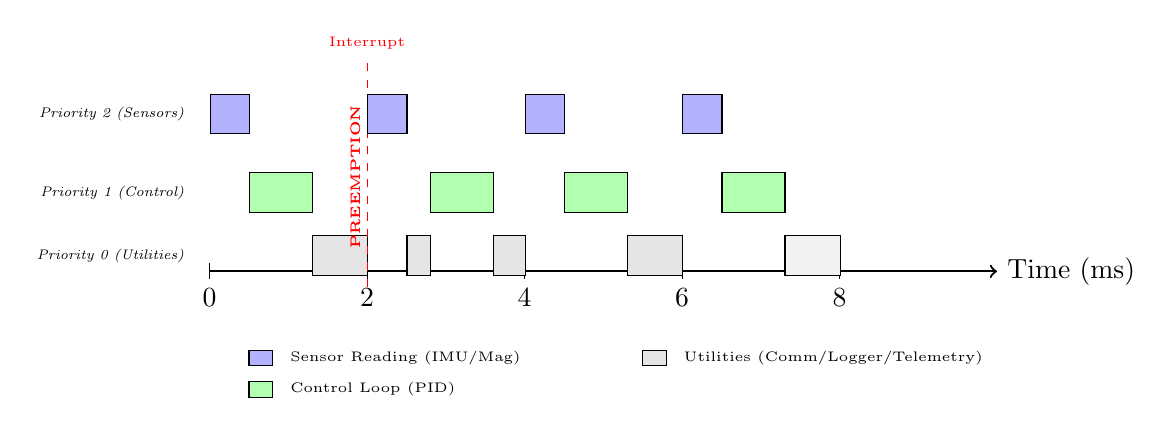
\begin{tikzpicture}[
        task/.style={draw, rectangle, minimum height=0.5cm, anchor=west},
        label/.style={font=\tiny\itshape, anchor=east},
        legend/.style={font=\tiny, anchor=west}
    ]

    % Time axis
    \draw[->, thick] (0,0) -- (10,0) node[right] {Time (ms)};
    \foreach \x in {0,2,4,6,8} \draw (\x,0.1) -- (\x,-0.1) node[below] {\x};

    % Priority Labels
    \node[label] at (-0.2, 2) {Priority 2 (Sensors)};
    \node[label] at (-0.2, 1) {Priority 1 (Control)};
    \node[label] at (-0.2, 0.2) {Priority 0 (Utilities)};

    % 0-2ms Cycle
    \node[task, fill=blue!30, minimum width=0.5cm] at (0, 2) {};
    \node[task, fill=green!30, minimum width=0.8cm] at (0.5, 1) {};
    \node[task, fill=gray!20, minimum width=0.7cm] at (1.3, 0.2) {};

    % 2-4ms Cycle (Showing Preemption)
    \draw[dashed, red] (2, -0.2) -- (2, 2.7) node[above, font=\tiny] {Interrupt};
    \node[task, fill=blue!30, minimum width=0.5cm] at (2, 2) {};
    
    % Resumed sequences
    \node[task, fill=gray!20, minimum width=0.3cm] at (2.5, 0.2) {}; 
    \node[task, fill=green!30, minimum width=0.8cm] at (2.8, 1) {};
    \node[task, fill=gray!20, minimum width=0.4cm] at (3.6, 0.2) {};

    % 4-6ms Cycle
    \node[task, fill=blue!30, minimum width=0.5cm] at (4, 2) {};
    \node[task, fill=green!30, minimum width=0.8cm] at (4.5, 1) {};
    \node[task, fill=gray!20, minimum width=0.7cm] at (5.3, 0.2) {};

    % 6-8ms Cycle
    \node[task, fill=blue!30, minimum width=0.5cm] at (6, 2) {};
    \node[task, fill=green!30, minimum width=0.8cm] at (6.5, 1) {};
    \node[task, fill=gray!10, minimum width=0.7cm] at (7.3, 0.2) {};

    % Legend (Two-column layout to prevent overlapping)
    \begin{scope}[shift={(0.5,-1.2)}]
        % Column 1
        \draw[fill=blue!30] (0,0) rectangle (0.3,0.2) node[legend] at (0.4,0.1) {Sensor Reading (IMU/Mag)};
        \draw[fill=green!30] (0,-0.4) rectangle (0.3,-0.2) node[legend] at (0.4,-0.3) {Control Loop (PID)};
        
        % Column 2
        \draw[fill=gray!20] (5,0) rectangle (5.3,0.2) node[legend] at (5.4,0.1) {Utilities (Comm/Logger/Telemetry)};
    \end{scope}

    % Preemption Highlight
    \node[text=red, rotate=90, font=\tiny\bfseries] at (1.85, 1.2) {PREEMPTION};

    \end{tikzpicture}
    \caption{Preemptive scheduling model of VAIOS, showing how sensor tasks interrupt lower-priority execution to ensure deterministic timing.}
    \label{fig:execution_timeline}
\end{figure}

\subsection{Deterministic Guarantees}

By utilizing a hardware-backed DWT (Data Watchpoint and Trace) timer and the VAIOS scheduler, the system achieves sub-microsecond jitter for task wakeup. This determinism is critical for the stability of the inner PID loop, where even a few milliseconds of variance in the sampling interval (\( dt \)) can lead to oscillations or loss of control during aggressive maneuvers.